\documentclass{article}
\title{Mean Shift Summary}
\author{Shuo Sun}
\date{07/09/2021}
\usepackage{amsmath}
\usepackage{graphicx}
\usepackage{subfigure}
% \usepackage{subfig}
\usepackage{subfloat}
\usepackage{lipsum}
\usepackage{float}

\usepackage[labelfont=it, textfont={bf,it}, font=small ]{caption}
% \usepackage{caption}
\usepackage{subcaption}
\usepackage[ruled, linesnumbered]{algorithm2e}
\usepackage{geometry}

\geometry{a4paper,scale=0.8}

\begin{document}

\maketitle

\section{Introduction}
\paragraph{
The Mean Shift(MS) algorithm is a kind of clustering algorithm based on density estimation. Given discretely sampled data, the MS algorithm aims to locate the maxima of the density function. To estimate the density function, one simple approach is to smooth the data, for example:
}
\begin{equation}
f(x) = \sum_{i=1}^{N}K(\frac{x-x_i}{h})
\end{equation}
\subparagraph{
where function K(x) is called the \textit{kernel function} if there exists a profile such that:
}
\begin{equation}
K(x) = k(||x||^2)
\end{equation}

\subparagraph{
the $k(x)$ should have the property:\\
1) $k$ in non-negative\\
2) $k$ is non-increasing: $k(a) \geq k(b)$ if $a < b$\\
3) $k$ is piece-wise continuous and $\int_{0}^{\infty}k(r)d(r) < \infty $
}

\subparagraph{
The sample mean with kernel K at $x \in X$ can be written as :
}

\begin{equation}
m(x) = \frac{\sum_{s\in S'}K(s-x)w(s)s}{\sum_{s \in S'}K(s-x)w(s)}
\end{equation}

\subparagraph{
where $S'$ is the a finite set(sample); $w(s)$ is the weight function.
}

\subparagraph{
Let $T \subset  X$ is a finite set, and we use the MS algorithm iteratively  $T \leftarrow m(T)$ until converging.  If the set $T = S$, we call it a blurring process.
}
\subparagraph{
Based on the above information, we can simply summarise the process of the Mean Shift algorithm:
}

\begin{algorithm}[t]
\caption{Mean Shift}
\KwIn{sample set: $S'$, point set: $T$, bandwidth: $h$, threshold: $\epsilon$}
\KwResult{shifting\_points set: $T'$}
i = 0\\
\For{$p_i$ in $T'$}{
    $p_{shift}$ \leftarrow $p_i$, $d$ \leftarrow \epsilon+\delta(\delta>0)\; \\
    \While{$d$ \le $\epsilon$}{
        $p_{old}$ \leftarrow $p_{shift}$\;\\
        $p_{new}$ \leftarrow GetNewPoint$(p_{old}, T)$\;\\
        $d$ \leftarrow $d(p_{old}, p_{new})$\;\\
        $p_{shift}$ \leftarrow $p_{new}$
    }
    $T'[i]$ = $p_{shift}$\;\\
    i += 1\;\\
}
\end{algorithm}


\subparagraph{
In this task, I give two different ways for the Mean-Shift algorithm to process circular-linear data. The difference between the two ways is how to compute the evaluate the distance between two points with $(\theta, r)$ format. The first one (Algo1) converts the point in polar coordinate to Cartesian coordinate. The second one (Algo2) directly computes the distance between two points like Euclidean space.
}

%---------------------------------- section 2 ------------------------------------------------%
\section{Methods}

\subsection{Distance between points}
\paragraph{
When we use the kernel function to estimate the density around the point $x$:
}
\begin{equation}
f(x) = \sum_{i=1}^{N}K(\frac{x-x_i}{h})
\end{equation}
\subparagraph{
In the above equation, $(x-x_i)$ is used to describe the \textit{distance} between points. Different ways of evaluating the distance can result in different density functions. So the first thing to do is how to evaluate the distance between two points of circular-linear data.
}

\subsubsection{Algo1}
\paragraph{
The data given is circular-linear data, with the format$(\theta, r)$. The variable $\theta$ represents direction, and the variable $r$ represents the size in the direction. It is an intuitive idea that we can convert a vector in polar coordinate to a point in Cartesian coordinate:
}

\begin{equation}
\begin{aligned}
x = r \cos{\theta} \\
y = r \sin {\theta}
\end{aligned}
\end{equation}

\subparagraph{
We are familiar with the distance between two points in Cartesian coordinate:
}

\begin{equation}
d(p_{1}, p_{2}) = \sqrt{(x_{1} - x_{2})^2 + ({y_1 - y_2})^2}
\end{equation}

\subparagraph{
After getting the data with the format of $(\theta,r)$, the data should be pre-processed first. The set after processed is called $S_p$. In the successive steps, the data set $S_p$ will be used to find clusters.
}

\subsubsection{Algo2}
\paragraph{
We can also compute the distance directly on the raw data in a way similar to Cartesian coordinate:
}

\begin{equation}
d(p_1, p_2) = \sqrt{({\theta_1 - \theta_2})^2 + ({r_1 - r_2})^2}
\end{equation}

\subparagraph{
However, the variable $\theta$ is angle in $[0, 2 \pi]$, the angle is a kind of periodic value. That means the real distance between $0$ and $2\pi$ is $0$ , not $2\pi$. Similarly, the distance between $0$ and $\frac{3}{2} \pi$ is $\frac{1}{2} \pi$. As shown below:
\begin{figure}[H]
    \centering
    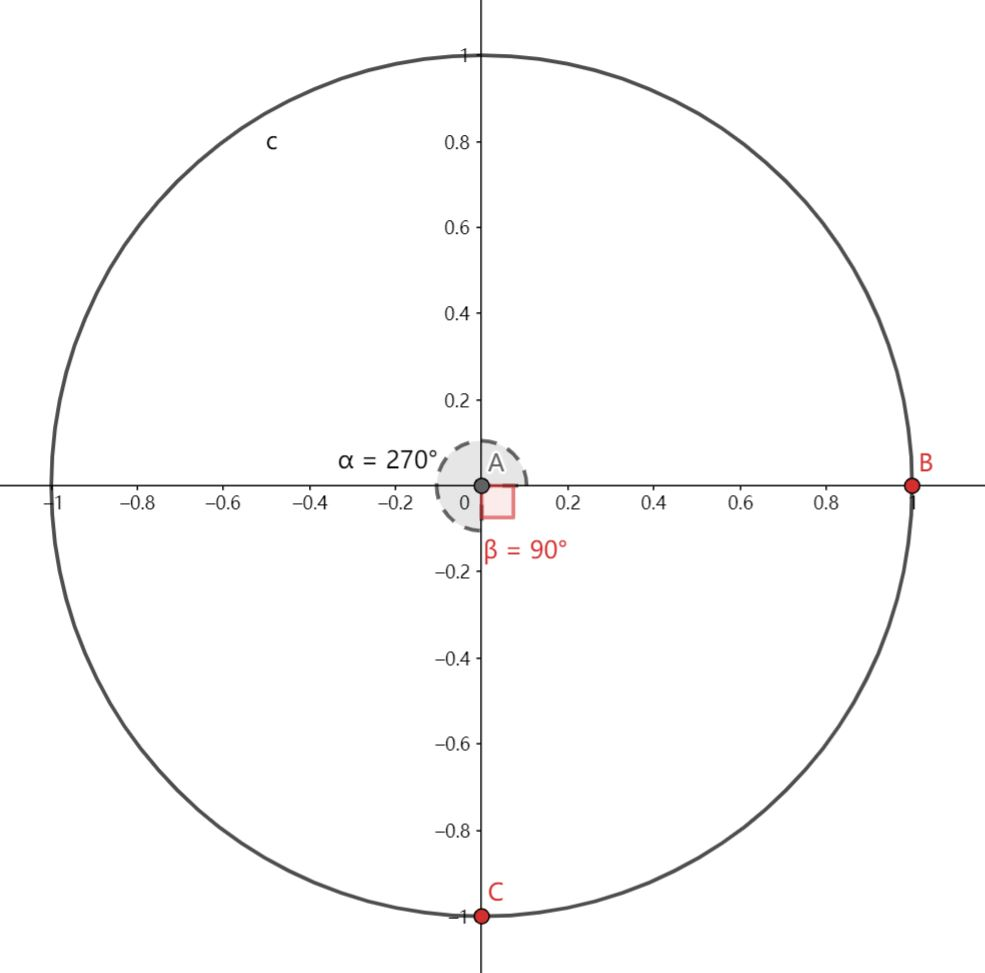
\includegraphics[width=6cm]{0-23}
    \caption{Point B represents $0$, point C represents $3\pi/2$, the real \textit{distance} between B and C is {$\pi$}/{2}}
\end{figure}
}

\subparagraph{
    So, the distance between the two angles should be:
}

\begin{equation}
    d(\theta_1, \theta_2) =
    \begin{cases}
    2\pi - |\theta_1 - \theta_2| &|\theta_1 - \theta_2|>\pi\\
    |\theta_1 - \theta_2|  &else
    \end{cases}
\end{equation}

\subparagraph{
    The distance of the circular-linear data is:
}

\begin{equation}
    d(v_1,v_2) = \sqrt{d^2(\theta_1 - \theta_2) + (r_1 - r_2)^2}
\end{equation}

% -------------------The section 2-------------------%
\subsection{Parameters choosing}
\subsubsection{Bandwidth}
\paragraph{
    The main parameter of the Mean Shift algorithm is the \textit{bandwidth} of the kernel function.
    If h is small, the point with a larger distance will have a smaller weight. The fewer points will be used to estimate density, the variance will be larger. However, if h is large, this will result in a bigger bias.
    So, there is a trade-off between bias and variance when choosing bandwidth. Given the size of sampled data N, the bandwidth should meet the requirement that $N\rightarrow \infty$, $h \rightarrow 0$. By this, we can get h should be :
}

\begin{equation}
    h = cN^{-1/5}
\end{equation}
\subparagraph{
    where c is a constant.
}
\subparagraph{
    For the Gaussian distribution, $h$ should be:
}

\begin{equation}
\begin{aligned}
    h &= (\frac{4\sigma^5}{3N})^{1/5}
&=\frac{1.05 * \sigma}{N^5}
\end{aligned}
\end{equation}
\subparagraph{where $\sigma$ is the standard deviation for the sample.}

\subsubsection{Kernel Function}
\paragraph{
    The common kernel function used is \textit{flat kernel} :
}

\begin{equation}
    F(x) =
    \begin{cases}
        1 &if ||x|| \le h\\
        0 &if ||x|| > h
        \end{cases}
\end{equation}
\subparagraph{and \textit{Gaussian kernel}:}

\begin{equation}
    G(x) = \frac{1}{h\sqrt{2\pi}} e^{-\frac{||x||^2}{2h^2}}
\end{equation}

\subparagraph{
    The kernel function can be seen as the weight to estimate the point around $x$.
    The \textit{flat kernel} can be seen as a d-dimensional sphere, only the point in this sphere will be considered.
    The \textit{Gaussian kernel} consider all the points in the set, but closer points will have larger point.
}
\subparagraph{
    In this task, we will use the \textit{Gaussian kernel} as the kernel function.
}

\subsubsection{Weight Function}
\paragraph{
    Weight function $w(s)$ can be fixed or re-evaluated after each iteration. In this task, the Gaussian kernel has already
    set the weight for each point, so I just set $w(s) = 1$ in the iteration.
}

\subsubsection{Threshold}
\paragraph{
    The parameter threshold is used to decide when to stop the iteration. The larger threshold will result in more clusters. But smaller thresholds may result in
    that there is only one mode in the set. In this task, we will set different threshold and analyse the results.
}

%-------------------------section 3----------------------------%
\section{Data Analysis}
%----------section 3.1
\subsection{Computing Means}
\paragraph{
    After the iteration of Mean Shift algorithm, we can get different modes of data. To estimate the basic parameters of different modes,
    we need to find the centre of each cluster by computing the mean point of each cluster.
}
\subparagraph{
    The simplest idea is $\bar{x} = \frac{1}{N} \sum_{i}^N{x_i}$. For $\theta$, it can be seen as a point on a unit circle. We can cut the circle and make it a line:
    \begin{figure}[H]
        \begin{subfigure}
          \centering
          % include first image
          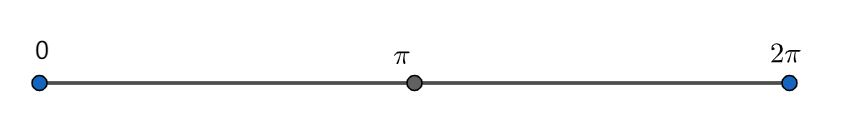
\includegraphics[width=.8\linewidth]{line.JPG}
          \caption{Cut from $\pi$}
          \label{fig:sub-first}
        \end{subfigure}
        \begin{subfigure}
          \centering
          % include second image
          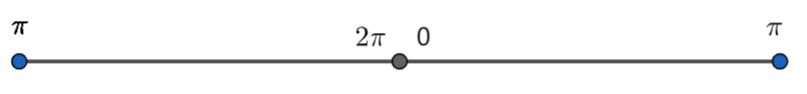
\includegraphics[width=.8\linewidth]{line2.JPG}
          \caption{Cut from $0$}
          \label{fig:sub-second}
        \end{subfigure}
    \end{figure}
    }


\subparagraph{
By choosing the point where to cut, we can also get different lines. So, the cutting point may have an effect on the out result.
}

\subparagraph{
Based on the \textit{Algo1}, we can also convert the point to Cartesian coordinate $[x,y]^T = [\cos(\theta), \sin(\theta)]^T$. So we can compute the mean value of each axis separately by :
}

\begin{equation}
\begin{aligned}
\bar{c} = \frac{1}{N} \sum_{i}^{N}\cos{\theta_{i}} \\
\bar{s} = \frac{1}{N} \sum_{i}^{N}\sin{\theta_{i}}
\end{aligned}
\end{equation}

\subparagraph{
So, we can get the centre of the cluster, for its $\theta_c$ variable, it has the format:
}

\begin{equation}
    \begin{aligned}
    \cos(\theta_c) = \bar{c} = \frac{1}{N} \sum_{i}^{N}\cos{\theta_{i}} \\
    \sin(\theta_c) = \bar{s} = \frac{1}{N} \sum_{i}^{N}\sin{\theta_{i}}
    \end{aligned}
\end{equation}

\subparagraph{
Back to the $\theta$:
}

\begin{equation}
\theta_c =
    \begin{cases}
        \arctan{(\frac{\sin{\theta_c}}{\cos{\theta_c}})} &if \cos{\theta_c} >0\\
        arctan{(\frac{\sin{\theta_c}}{\cos{\theta_c}})}+\pi &if \cos{\theta_c} <0
    \end{cases}
\end{equation}

\subparagraph{
For the radius $r$, we can just compute it by :
}

\begin{equation}
    \bar{r} = \sum_{i}^{N}r_i
\end{equation}

%----------section 3.2
\subsection{Computing Variance}
\subparagraph{
Variance is a measure of dispersion, based on the meaning of distance of two circular-linear points, we compute the variance in the distance space:
}
\begin{equation}
    \begin{aligned}
    \sigma^2 &= \frac{1}{N-1}\sum_{i=1}^{N}(p_i - p_c)^2\\
            &=\frac{1}{N-1}\sum_{i=1}^{N}d(p_i, p_c)^2
    \end{aligned}
\end{equation}

%--------------------section 4-----------------------------------%
\section{Conclusion}
\subsection{Clustering results of given data}
\paragraph{
Here, I set some basic parameters as the baseline:\\
1) $h$ (bandwidth) is set by the equation(11);\\
2) $\epsilon$ (threshold) = 0.00001\;\\
3) $cluster\_distance$ (to identify points) = 0.5
}

\subparagraph{
The results are shown as below,
}

\subparagraph{
\begin{figure}[H]
    \centering
    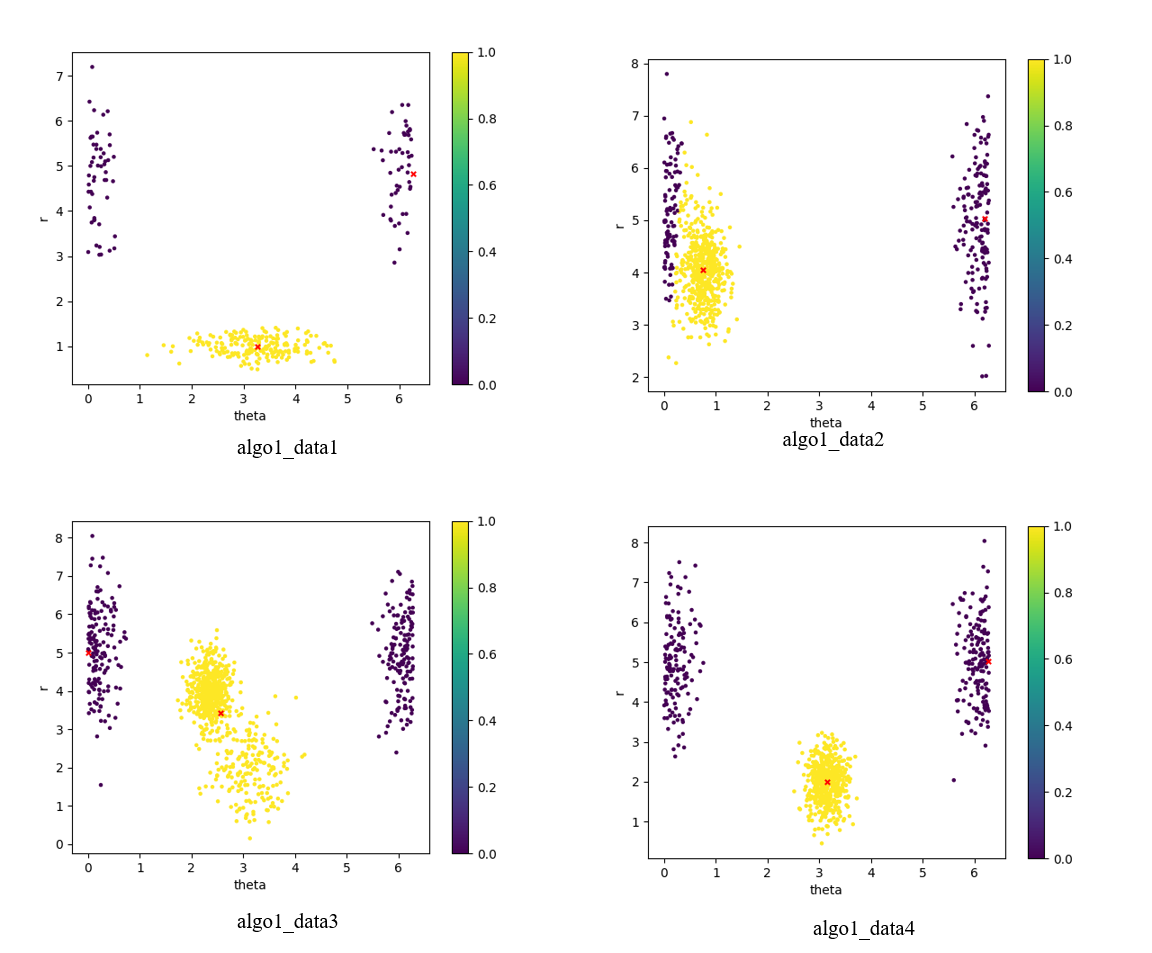
\includegraphics[width=11cm]{algo1.png}
    \caption{The clustering results used algorithm1}
\end{figure}
}

\subparagraph{
\begin{figure}[H]
    \centering
    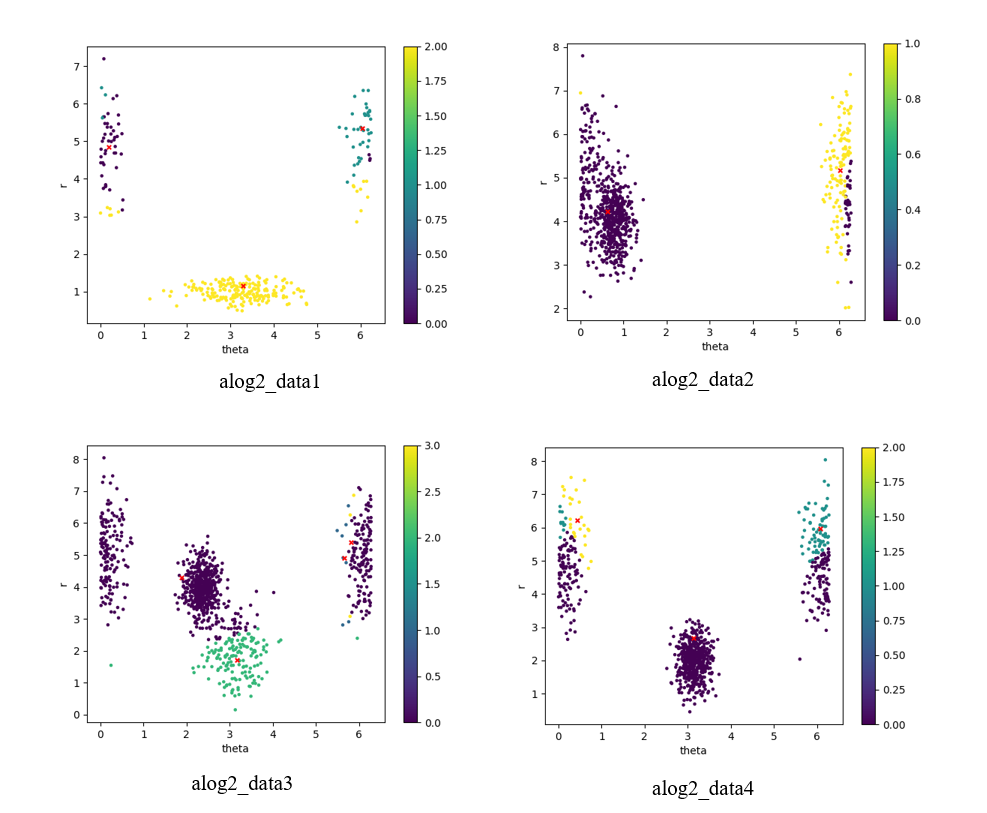
\includegraphics[width=11cm]{algo2.png}
    \caption{The clustering results used algorithm2}
\end{figure}
}


\subparagraph{
The corresponding parameters are:
}
\subparagraph{
For \textit{Algo1}:\\
1)\textit{Algo1\_data1}:\\
Mean1, variance1 = [6.264581278374883, 4.835123552413281], 0.939911335274201\\
Mean2, variance2 = [3.260652115284019, 0.9951555487518141], 0.4847930143675687\\
2)\textit{Algo1\_data2}:\\
Mean1, variance1 = [6.195806779743288, 5.038739483173911], 1.0144883862305363\\
Mean2, variance2 = [0.7578102016545607, 4.056523895407684], 0.43649180883735894\\
3)\textit{Algo1\_data3}:\\
Mean1, variance1 = [0.0011053485412668106, 5.008956198106666], 1.1546428427750621\\
Mean2, variance2 = [2.561818743211738, 3.4347695060328554], 1.345255056792747\\
4)\textit{Algo1\_data4}:\\
Mean1, variance1 = [6.275052766052679, 5.0138292362733345], 1.126485967720785\\
Mean2, variance2 = [3.1462162642512377, 1.985775081232], 0.28859923244214547
}
\subparagraph{
For \textit{Algo2}:\\
1)\textit{Algo2\_data1}:\\
Mean1, variance1 = [0.20222136352012238, 4.854327167542238], 0.6226003937141277\\
Mean2, variance2 = [6.042231988296247, 5.349348037649856], 0.43750127152496493\\
Mean3, variance3 = [3.2814843637511655, 1.1633712602153288], 1.4042334165883408\\
2)\textit{Algo2\_data2}:\\
Mean1, variance1 = [0.6241342718010923, 4.22775436941789], 0.7075564329703974\\
Mean2, variance2 = [6.017494334803616, 5.172806610915254], 1.1435871536830982\\
3)\textit{Algo2\_data3}:\\
Mean1, variance1 = [1.8852498215398534, 4.291848884517322], 2.301119305564973\\
Mean2, variance2 = [5.660576532243779, 4.90552073475], 1.923843711654354\\
Mean3, variance3 = [3.1683116862320397, 1.7059184362171056], 0.537530802469436\\
Mean4, variance4 = [5.82388720943778, 5.401409710333334], 4.150890959672452\\
4)\textit{Algo2\_data4}:\\
Mean1, variance1 = [3.138574735333872, 2.667478984917632], 3.954162764034368\\
Mean2, variance2 = [6.0711038101168135, 5.9668292419135796], 0.3574547782738188\\
Mean3, variance3 = [0.43445628507695205, 6.215840197777778], 0.6251928397153621
}

\subsection{Parameters effects}
\paragraph{
    Use data1 as the sampled set, Algo1 as the algorithm, threshold = 0.0001;
    The results with different bandwidth are shown below:
    \begin{figure}[H]
        \centering
        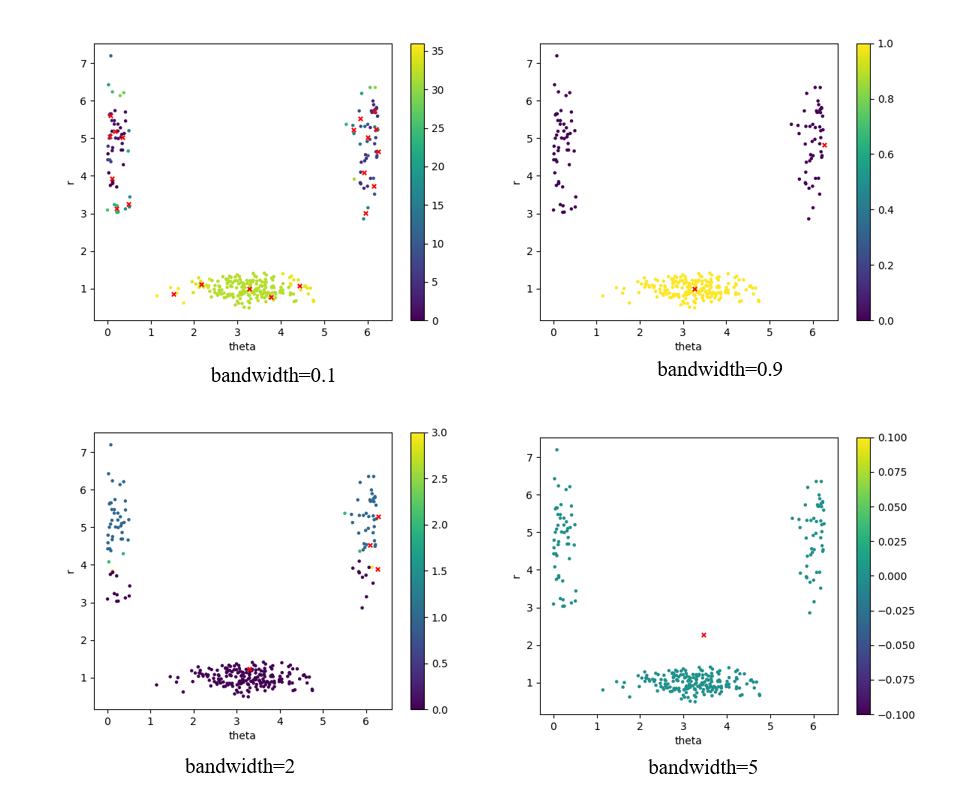
\includegraphics[width=10cm]{algo1_bandwidth.png}
        \caption{Different bandwidth}
    \end{figure}
}

\subparagraph{
    Use data1 as the sampled set, Algo1 as the algorithm, bandwidth = 0.9;
    The results with different threshold are shown below:
    \begin{figure}[H]
        \centering
        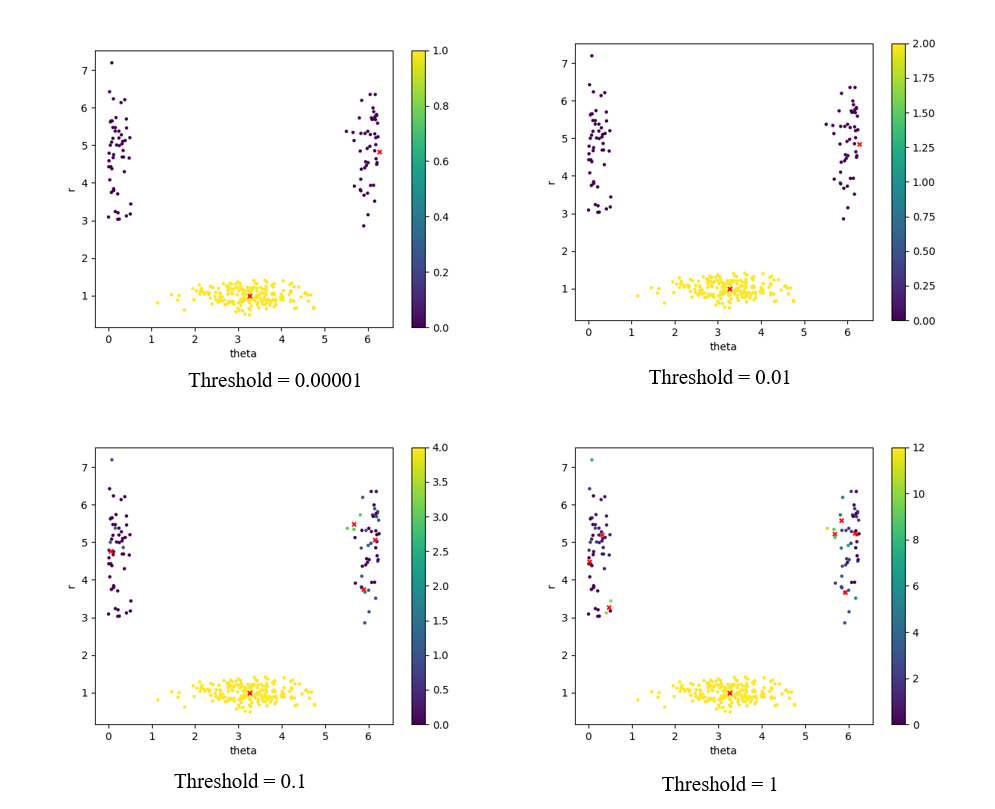
\includegraphics[width=10cm]{algo1_threshold.png}
        \caption{Different bandwidth}
    \end{figure}
}


\end{document}